


% ------------------ DOCUMENT SETUP ------------------ 
% The document class defines the document type (report) and sets the font size (10pt)
\documentclass[10pt]{report}
\author{Felipe Santos Almeida}

% Inputs the Document Packages
% ------------------ PACKAGES ------------------ 
% Packages add extra commands and features to your LaTeX document. 
% In here, some of the most common packages for a thesis document have been added 

% LaTeX's float package
\usepackage{float}

% LaTeX's color package
\usepackage{color}

% LaTeX's main math package
\usepackage{amsmath}

% LaTeX's Caption and subcaption packages
\usepackage[format=hang,font=normalsize,labelfont=bf,labelsep=colon,singlelinecheck=off]{caption}
\usepackage{subcaption}

% The graphicx package provides graphics support for adding pictures.
\usepackage{graphicx}

% Longtable allows you to write tables that continue to the next page.
\usepackage{longtable}

% The geometry packages defines the page layout (page dimensions, margins, etc)
\usepackage[a4 paper, top=25mm, bottom=25mm]{geometry}

% Defines the Font of the document, e.g. Arimo font (Check Fonts here: https://tug.org/FontCatalogue/)
\usepackage[sfdefault]{arimo}

% Font encoding
\usepackage[T1]{fontenc}

% This package allows the user to specify the input encoding
\usepackage[utf8]{inputenc}

% This package allows you to add empty pages
\usepackage{emptypage}

% Allows inputs to be imported from a directory
\usepackage{import}

% Provides control over the typography of the Table of Contents, List of Figures and List of Tables
\usepackage{tocloft}

% The setspace package controls the line spacing properties.
\usepackage{setspace}

% Allows the customization of Latex's title styles
\usepackage{titlesec}

% Allows the customization of Latex's table of contents title styles
\usepackage{titletoc}

% The package provides functions that offer alternative ways of implementing some LATEX kernel commands
\usepackage{etoolbox}

% Provides extensive facilities for constructing and controlling headers and footers
\usepackage{fancyhdr} 

% Typographical extensions, namely character protrusion, font expansion, adjustment 
%of interword spacing and additional kerning
\usepackage{microtype}

% Manages hyperlinks 
\usepackage[colorlinks=true,linkcolor=black,urlcolor=blue]{hyperref}

% Generates PDF bookmarks
\usepackage{bookmark}

% Add color to Tables
\usepackage[table,xcdraw]{xcolor}

% Use these two packages together -- they define symbols
%  for e.g. units that you can use in both text and math mode.
\usepackage{gensymb}
\usepackage{textcomp}

% Bibliography package
\usepackage[backend=biber,style=nature]{biblatex}
\addbibresource{references.bib} % Add the .bib file that contains the references

% The natbib package allows book-type citations (e.g. (Saucer et al., 1993))
% More details are here: http://merkel.zoneo.net/Latex/natbib.php
%\usepackage[round]{natbib}

% The linenumbers command adds line numbers next to your text 
% That can be useful for discussing edits in drafts.
%\usepackage[modulo]{lineno}
%\linenumbers 


% This package provides an easy way to input latin sample text (for the template only)
\usepackage{blindtext}


\usepackage{booktabs}

% Controls how many subsections the document can take
%  and how many of those will get put into the contents pages.
\setcounter{secnumdepth}{2}
\setcounter{tocdepth}{2}

% Line Spacing
\setstretch{1.0}

% The folder path where the images will be uploaded
\graphicspath{{./Images/}} 

% Places a dot after Chapter/Section/Subsection number in Table of Contents
\renewcommand{\cftchapaftersnum}{.}
\renewcommand{\cftsecaftersnum}{.}
\renewcommand{\cftsubsecaftersnum}{.}

%  Customize Dot spacing in Table of Contents/List of Figures/Tables
\renewcommand{\cftdotsep}{0.3}

% Numeration Type for Chapters and Sections (Roman I, II, II / Arabic 1, 2, 3)
\renewcommand\thechapter{\Roman{chapter}}
\renewcommand\thesection{\arabic{section}}

% Line Break Properties
\tolerance=1
\emergencystretch=\maxdimen
\hyphenpenalty=10000
\hbadness=10000


% Formatting Table of Contents/Lists titles
\renewcommand{\contentsname}{\normalfont\bfseries\LARGE{CONTENTS}}
\renewcommand{\listfigurename}{\normalfont\bfseries\LARGE{LIST OF FIGURES}}
\renewcommand{\listtablename}{\normalfont\bfseries\LARGE{LIST OF TABLES}}


% Title Formatting customization
\titleformat{\chapter}{\normalfont\bfseries\LARGE}{\thechapter.}{1em}{\MakeUppercase}

\titleformat{\section}{\normalfont\bfseries\large}{\thesection.}{1em}{\MakeUppercase}
\titlespacing*{\section} {0pt} {0pt} {15pt} % left, before, after

\titleformat{\subsection}{\normalfont\bfseries\large}{\thesubsection.}{1em}{}
\titlespacing*{\subsection} {0pt} {10pt} {10pt}

\titleformat{\subsubsection}{\normalfont\bfseries\large}{}{1em}{}
\titlespacing*{\subsubsection} {0pt} {10pt} {10pt}


% HEADER AND FOOTER
\pagestyle{fancy}  % Set Page Style (Header and Footer Style)
\fancyhf{}  % Clears the header and footer (from the default info)

% Header
\renewcommand{\headrulewidth}{0pt}  % Removes the default Horizontal Line in Header
\fancyhead[L]{SN21125032}
\fancyhead[R]{May 2023}

% Footer
\fancyfoot[C]{\thepage} % Page Number

% Change figure numbering per section
\numberwithin{figure}{section}
\numberwithin{table}{section}






%  -------------------------------------------------
%  --------- The document starts from here --------- 
%  -------------------------------------------------

\begin{document}

% -------------------  INTRODUCTION  ---------------------

\begin{center}
    % UCL IMAGE
    \vspace*{-3cm}
    \makebox[\textwidth]{
\includegraphics[width=\paperwidth]{Image/UCL_LOGO_new.png}}
\end{center}   
    % Title
    {\LARGE\textbf{Assessment\\
    % Subtitle
    CASA0002 – Urban Simulation\\}}
SN21125032 | Word count: 

\vspace{5mm} %5mm vertical space
  
\section{Part 1: London’s underground resilience}


 \subsection{Topological Network}
\subsubsection{Centrality Measures } 
        
         Aiming to evaluate the resilience of the Tube Network and the impact of node removals, the three centralities measures chosen to identify the most important nodes in the Tube Network are Degree, Eigenvector, and Betweenness centrality. The first experiment of this analysis was also considered to use closeness centrality. However, the application in the context of node removal in this centrality measures has not presented good results.  
        
        \vspace{5mm} %5mm vertical space
        
        \textbf{Degree Centrality:} The number of links associated with a node related to the tube network(Figure \ref{fig:Part1_topologicalmap_degree}). This centrality reflects the number of connections with a station, which can be linked with another station or tube line that starts and finish in the same station, as a loop, for example. Regarding this analysis, the degree centrality values are normalised by dividing them by the maximum possible degree, which is n-1. 

    \begin{figure}[htp]
        \centering
        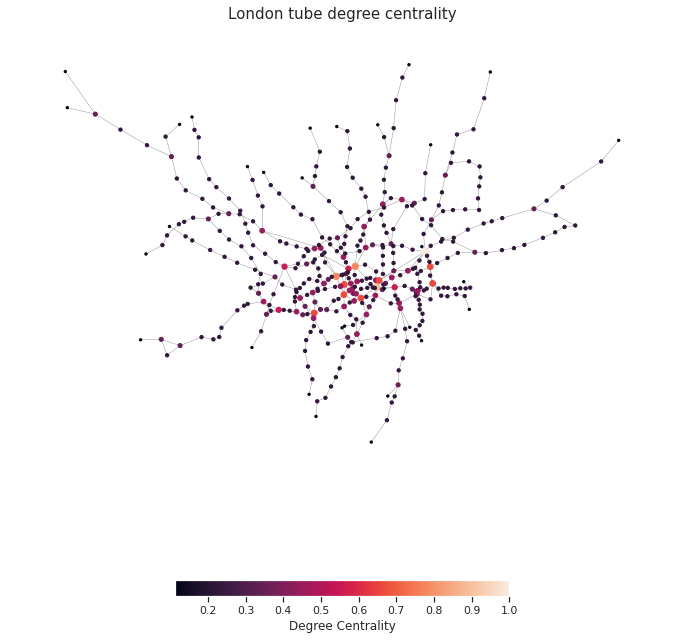
\includegraphics[width=12cm]{Image/Part1_topologicalmap_degree.png}
        \caption{Topological Tube network map - Degree centrality}
        \label{fig:Part1_topologicalmap_degree}
    \end{figure}   


        
\newpage  
        
        \textbf{Eigenvector centrality:}  The transitive influence of nodes(Figure \ref{fig:Part1_topologicalmap_eigenvector}). Eigenvector centrality measures the influence of a node in a network based on a relative score for all nodes. Thus, nodes with a high-score mean that these nodes are also connected to other nodes with a high score. For tube network, these measure is useful because it is possible to understand the influence of a tube station not only focused on its good connectivity with a  range of tube lines. This centrality allows us to understand how good is the connectivity of the neighbour's stations. Therefore, when it is considered a station disruption, an individual close to other stations is well-connected to improve the user experience in the system. 

    \vspace{5mm} %5mm vertical space    
        
    \begin{figure}[htp]
        \centering
        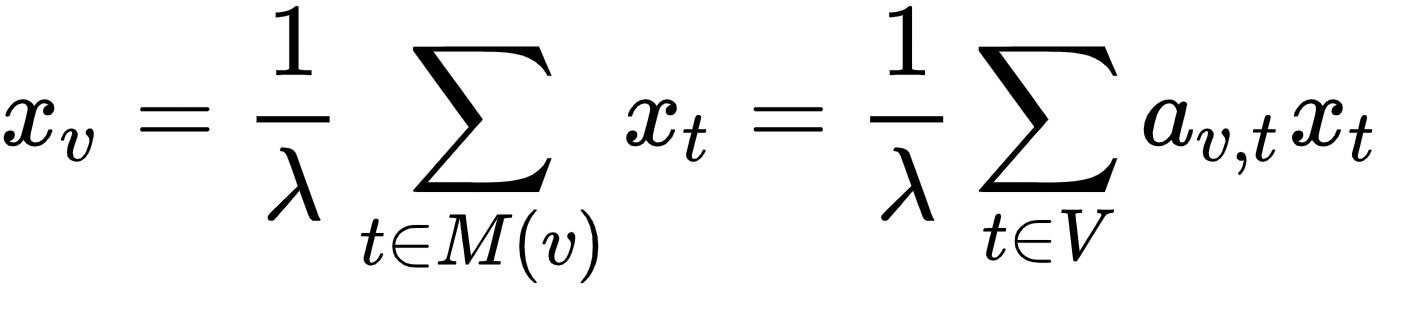
\includegraphics[width=5cm]{Image/eigenvector equation.jpeg}
        \caption{Eigenvector centrality - Equation}
        \label{fig:eigenvector equation}
    \end{figure} 

        
    \begin{figure}[htp]
        \centering
        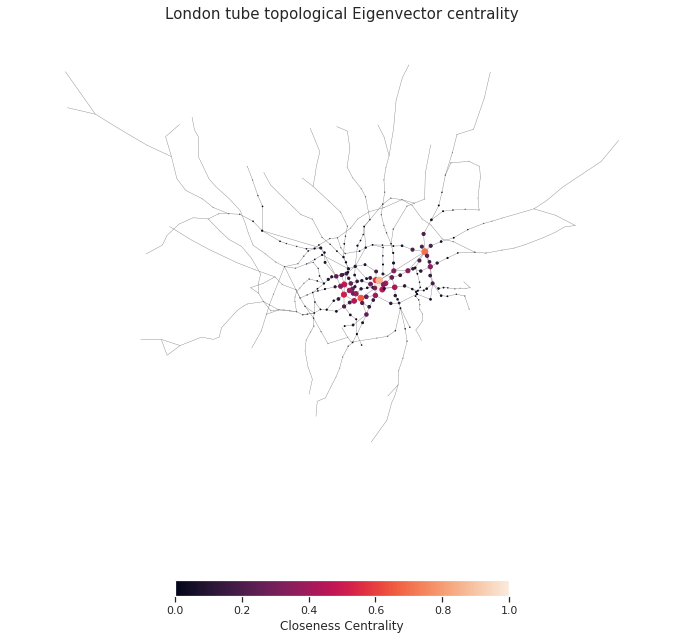
\includegraphics[width=14cm]{Image/Part1_topologicalmap_eigenvector.png}
        \caption{Topological Tube network map - Eigenvector centrality}
        \label{fig:Part1_topologicalmap_eigenvector}
    \end{figure} 

  
\newpage   
        \textbf{Betweenness centrality:} The shortest path passing through a node( Figure \ref{fig:Part1_topologicalmap_betweenness}). It is possible to detect the level of influence a node has on the flow of information. Thus, it can find the nodes that bridge a different part of the network. Related to the tube network, this measure is an essential outcome for understanding which tube station has the characteristic to allow users to commute easily and fast into the system.
        
        To calculate the betweenness centrality of a node is the sum of all shortest paths that pass through the vertex, where 
                    

\begin{equation}x_{i}=\sum_{st} \frac {n^{i}_{st}}{g_{st}}\end{equation}
        
    \begin{figure}[htp]
        \centering
        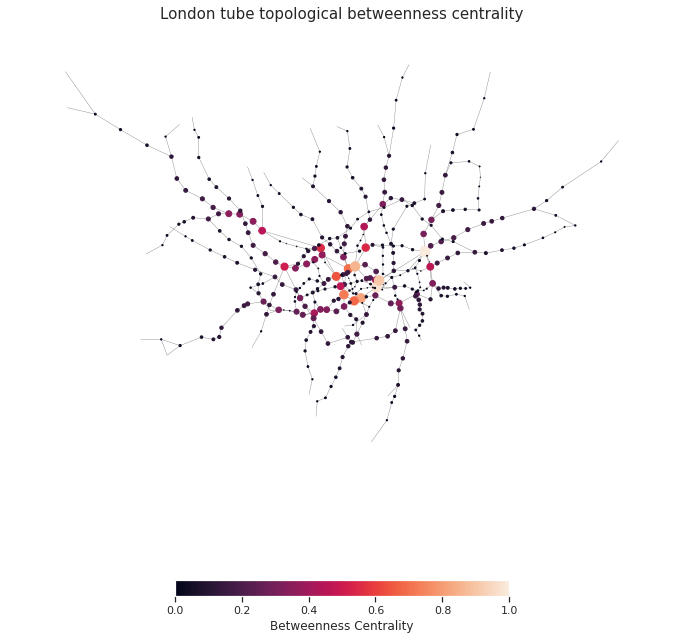
\includegraphics[width=14cm]{Image/Part1_topologicalmap_betweenness.png}
        \caption{Topological Tube network map - Betweenness centrality}
        \label{fig:Part1_topologicalmap_betweenness}
    \end{figure} 

  \vspace{5mm} %5mm vertical space

    To summarise( Figura \ref{fig:Table_CentralitiesMeasures}), Stratford is the station with the highest degree and betweenness topological centrality in London's Tube Network, while Bank and Monument is the node with the highest eigenvector centrality. Overall, Stratford, Bank and Monument and Liverpool Street represent a significant position in the three rankings, showing a concentration of important nodes in London's central/east region. All the values are normalised to allow a comparison among measures.  

    \begin{figure}[htp]
        \centering
        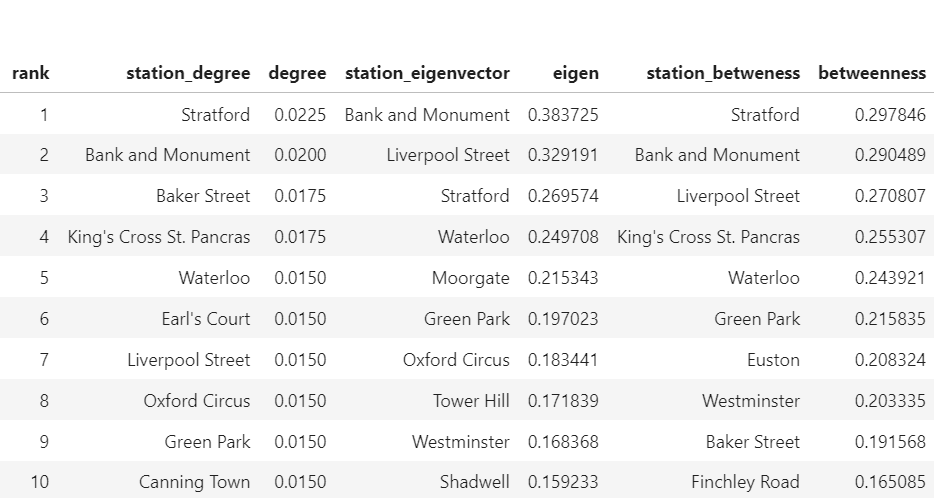
\includegraphics[width=14cm]{Image/Table_CentralitiesMeasures.png}
        \caption{Centrality measures}
        \label{fig:Table_CentralitiesMeasures}
    \end{figure}

\newpage    

\subsubsection{Impact Measures} 

In order to evaluate the topological network and use this measure to evaluate the removal of stations, this analysis uses the Size Largest Component and the Number of Components. The current network has only 1 component. However, when the stations start to be removed, some links will be disconnected, and the number of components will increase. Thus, it is crucial to choose measures that can detect the impact of removing that station, considering the rearrangement of the topological network. 

\subsubsection{Node Removal} 

In order to measure the impact of nodes removal in sequential and non-sequential order, a was developed a loop through values of n from 0 to 10 and then stored the results of the number of nodes removed, the impact measures, the total o nodes and consequently, which station was removed from the system. Thus, this process was applied to the three centrality measures and merged into a unique dataset. Therefore, it is possible to analyse the impact of node removal in the graphs below ( Figure \ref{fig:Part1_nonsequential_Summarise}). 


    \begin{figure}[htp]
        \centering
        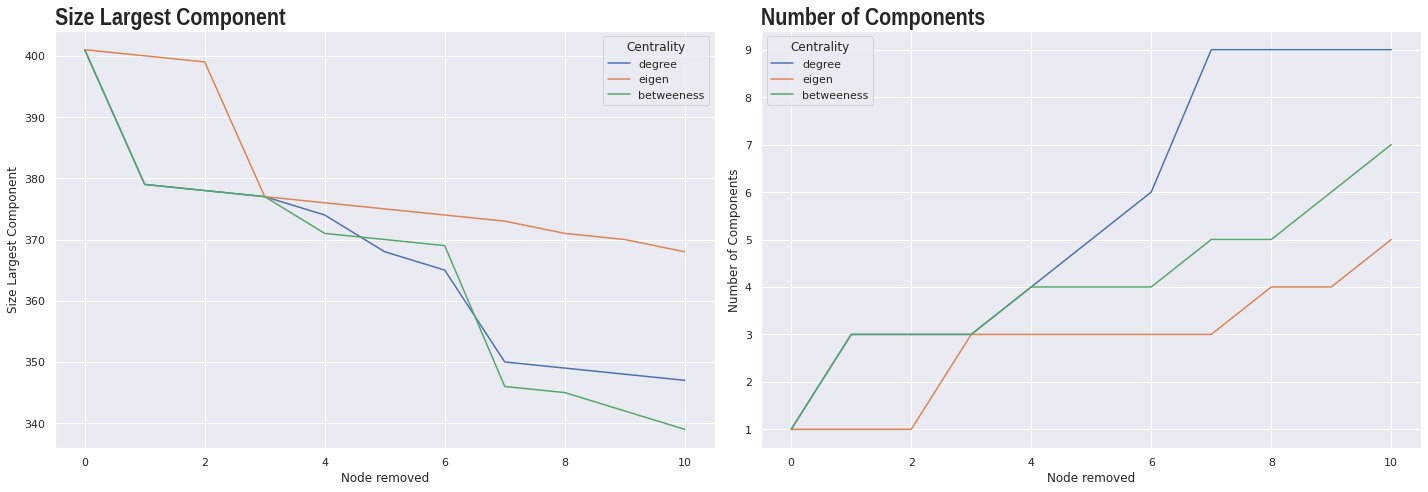
\includegraphics[width=16cm]{Image/Part1_nonsequential_Summarise.png}
        \caption{Non-sequential node removal}
        \label{fig:Part1_nonsequential_Summarise}
    \end{figure}

For the sequential removal nodes( Figure \ref{fig:Part1_sequential_Summarise}),  betweenness centrality had a sharp drop in the sizer of the largest component after removing the 6th node in the system( Green Park). The largest component's size variation remained around the initial value in the other centralities without drastic drops or increases. 

    \begin{figure}[htp]
        \centering
        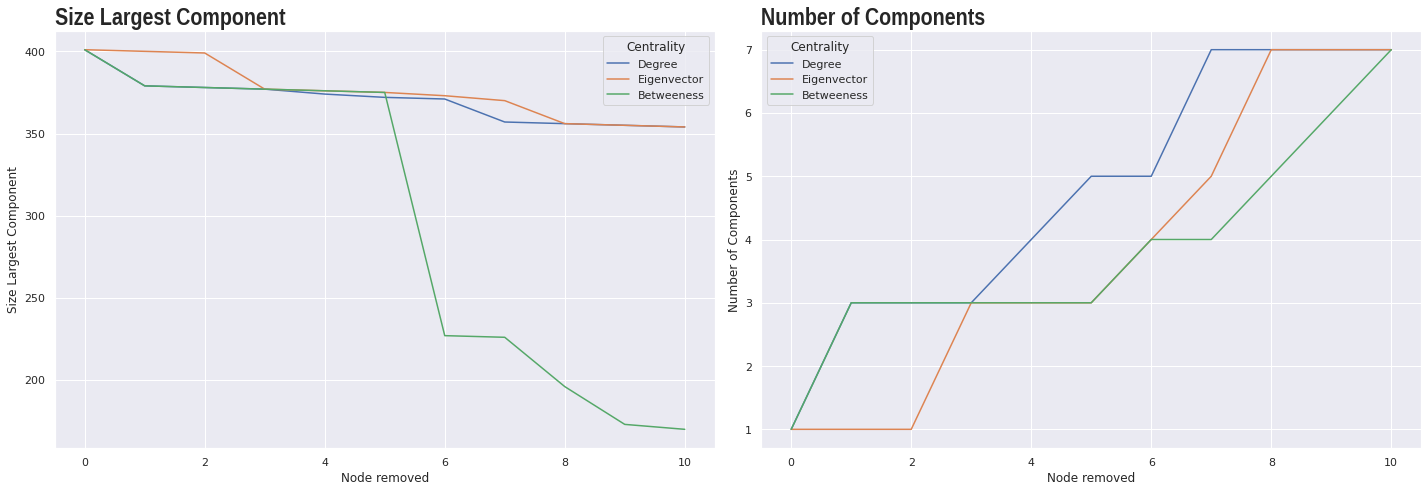
\includegraphics[width=16cm]{Image/Part1_sequential_Summarise.png}
        \caption{Sequential node removal}
        \label{fig:Part1_sequential_Summarise}
    \end{figure}


\newpage

\subsection{Flows: weighted network} 

\subsubsection{Centrality Measures } 

The weighted network outcomes performed a different ranking behaviour, mainly for the betweenness centrality. \textit{West Hampstead}, \textit{Gospel Oak} and \textit{Finchley Road \& Frognal} are stations that were not present in the topological network ranking( Figure \ref{fig:Table_CentralitiesMeasures_Flows}). 

    \begin{figure}[htp]
        \centering
        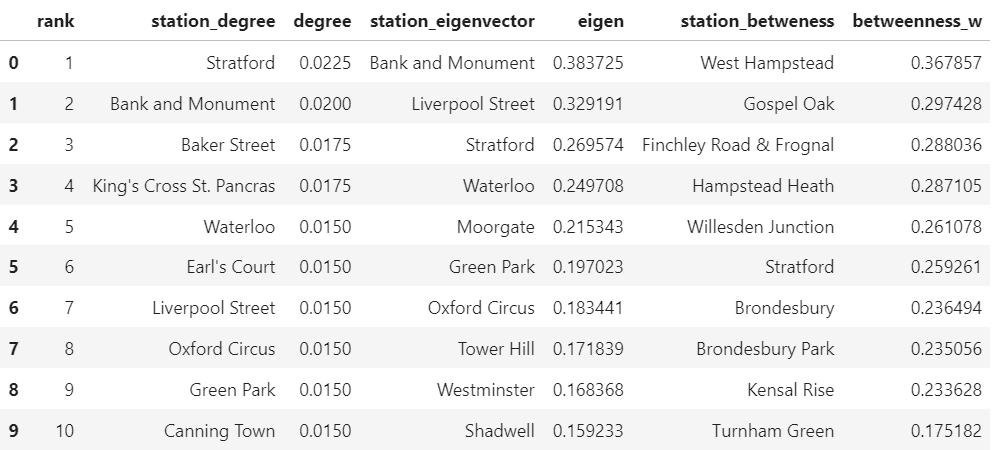
\includegraphics[width=14cm]{Image/Table_CentralitiesMeasures_Flows.png}
        \caption{Flows - Centrality measures}
        \label{fig:Table_CentralitiesMeasures_Flows}
    \end{figure}


\subsubsection{Impact Measures} 

For this analysis, it will remain the number of component and size largest components, in addition to the Flows of the largest component. Aiming to understand the impact in the flows, removing a tube station. 

\newpage 

\subsubsection{Node Removal} 

The Degree centrality ranking, the measure number of components and the size largest component did not have different values. However, the flows of the largest component presented crucial information about the importance of removed stations in the networking flows(Figure \ref{fig:Table_Flows_degree}). 

    \begin{figure}[htp]
        \centering
        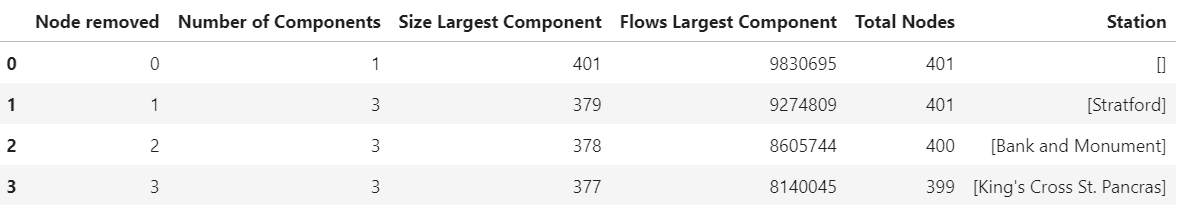
\includegraphics[width=14cm]{Image/Table_Flows_degree.png}
        \caption{Weighted Network - Degree Centrality}
        \label{fig:Table_Flows_degree}
    \end{figure}

For eigenvector centrality, Stratford station caused one of the highest impacts on the flow in the network, removing a considerable amount of flow in addition to separating the network into three components( Figure \ref{fig:Table_Flows_eigenvector}).

    \begin{figure}[htp]
        \centering
        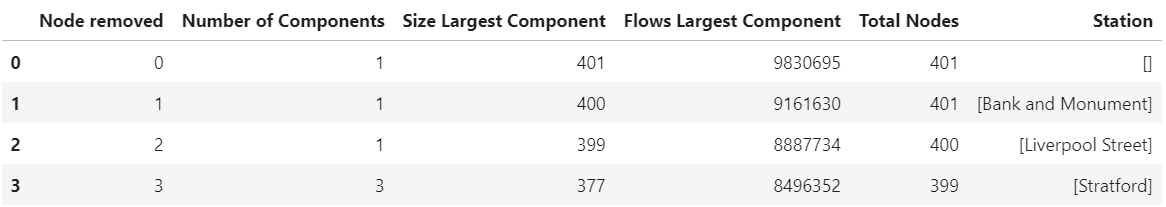
\includegraphics[width=14cm]{Image/Table_Flows_eigenvector.png}
        \caption{Weighted Network - Eigenvector Centrality}
        \label{fig:Table_Flows_eigenvector}
    \end{figure}

Although the betweenness centrality measure for Tube networking includes stations that differ from other centrality measures, removing these stations does not significantly impact the flow of network traffic or the size of the largest component. Consequently, when evaluating the resilience of the tube system by incorporating flows, betweenness centrality may not be a suitable centrality measure.

(Figure \ref{fig:Table_Flows_Betweenness}). 
    \begin{figure}[htp]
        \centering
        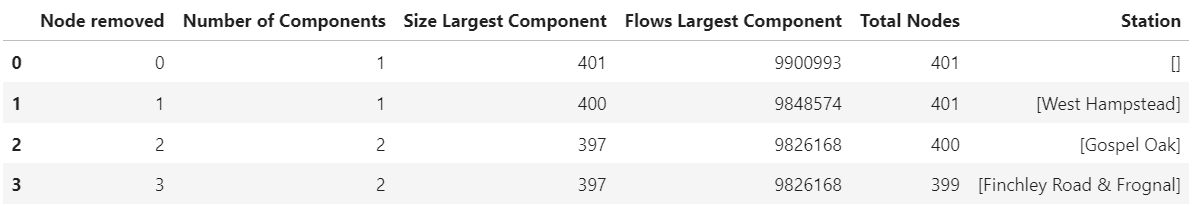
\includegraphics[width=14cm]{Image/Table_Flows_Betweenness.png}
        \caption{Weighted Network - Betweenness Centrality}
        \label{fig:Table_Flows_Betweenness}
    \end{figure}

Considering the significant impact observed with degree centrality and eigenvector centrality, it becomes apparent that Stratford, Bank and Monument, Liverpool Street, and King's Cross stations play crucial roles in facilitating user flows within the system during the specified period. Conversely, the size of the largest component and the number of components did not prove to be relevant measures for evaluating the flows in the system. However, these measures are still valuable for assessing the behaviour of other metrics, such as the flows within the largest component.

\newpage 

\section{ Part 2: Spatial Interaction models}

\subsection{Models and calibration}

Gravity Model( Unconstrained model), and the constrained models( Production-constrained Model, Attraction-Constrained Model and Doubly Constrained model)

\vspace{5mm} %5mm vertical space

\textbf{- Gravity model:}
The gravity model assumes the flows between the origin and destination are proportional to the mass of the origin and destination and inversely proportional to the distance between them. That means if the distance decreases, the flow increase and if the flows decrease, the origin and destination mass decrease.

\begin{equation} \tag{1}
T_{ij} = k O_i^\alpha  D_j^\gamma  d_{ij}^{-\beta}
\end{equation}

\vspace{5mm} %5mm vertical space

In unconstrained models, the constant K is employed to ensure the inclusion of all values. However, in constrained models, we can add the sums of origin and destination separately, providing greater flexibility to test the model in more specific scenarios. This allows for a more nuanced evaluation of the model's performance.

\vspace{5mm} %5mm vertical space

\textbf{- Production-Constrained Model:}

The Production(origin) Constrained Spatial Interaction Model is a powerful framework for understanding how origins behave and commute within a city to reach points of interest. These estimated flows can be connected to different variables related to these attractive points, such as budget and store size. In the context of London's tube network, the flows can be estimated using the equation below, which incorporates the logarithm of job values and the distance(cost).

\begin{equation} \label{eq:1} \tag{2}
T_{ij} = A_i O_i D_j^\gamma d_{ij}^{-\beta}
\end{equation}

\vspace{5mm} %5mm vertical space

\textbf{- Attraction-Constrained Model}

The Attraction(destination) Constrained model plays a crucial role in assessing the impact of a significant increase in demand within a specific region, such as establishing a new university or creating many job opportunities. By applying the value of this increase to the model, we can estimate how this new pattern will affect commuting flows and gain insights into the origins of these flows towards the destination. When applied to the tube network, the model considers the logarithm values of population, distance (cost), and destination stations,  resulting and the relationship of all these values with the flows in the system.


\begin{equation} \label{eq:5} \tag{3}
T_ij = D_j B_j O_i^\alpha d_{ij}^{-\beta}
\end{equation}

\vspace{5mm} %5mm vertical space
\textbf{- Doubly Constrained Model}
 In the doubly constrained model is only considered the flows. However, first,t it is crucial to detect a good beta. Thus, the beta is used to calculate the new origin and destination flows. Beta values do not change unless the mode of transport changes. 

\begin{equation} \tag{4}
T_{ij} = A_i B_j O_i D_j d_{ij}^{-\beta}
\end{equation}

\vspace{5mm} %5mm vertical space

Thus, the Production-constrained model was selected to analyse London's tube network. 

    \begin{figure}[htp]
        \centering
        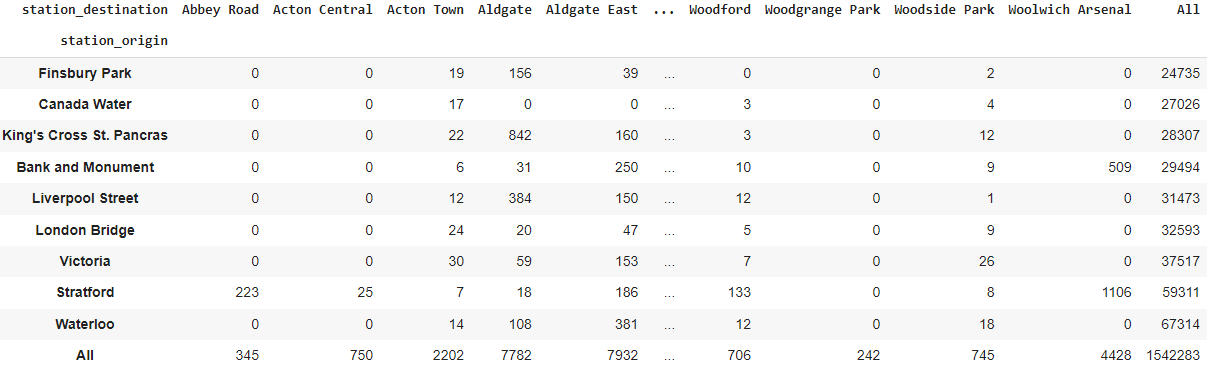
\includegraphics[width=16cm]{Image/Part2_OD.png}
        \caption{Model before calibration}
        \label{fig: Model before calibration}
    \end{figure}

In order to build the Production-constrained model, the following variables were applied in the equation: Flows, Jobs, Population and Distance as the cost. 

    \begin{figure}[htp]
        \centering
        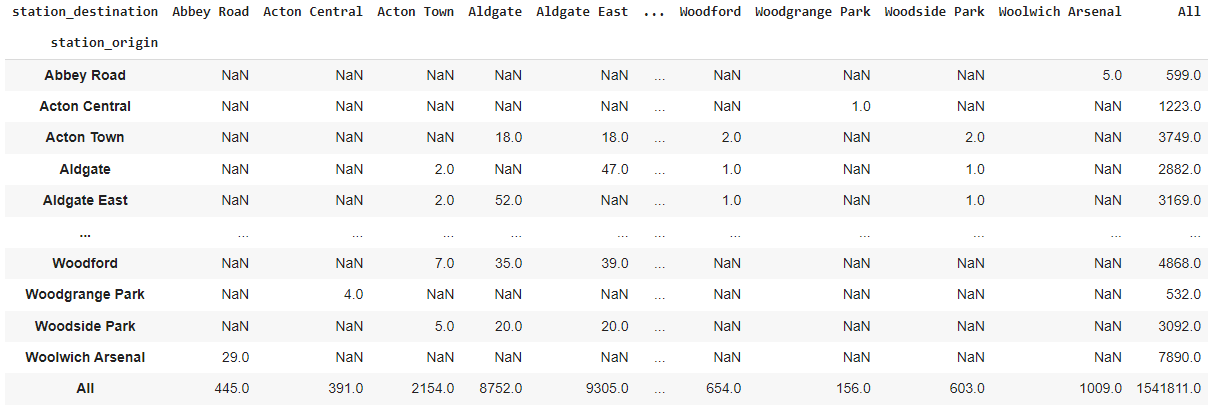
\includegraphics[width=16cm]{Image/Part2_OD2.png}
        \caption{Model after calibration}
        \label{fig: Model after calibration}
    \end{figure}

\newpage    

\subsection{Scenarios}
\subsubsection{Scenario A}

Assuming the Canary Wharf decreased in 50\% the total number of jobs, the flows were recalculated, reducing from 58,772 to 29,386. Thus, a new value for gamma and beta was calculated and then generated Ai value. As a result, the total number of flows only had a small variation. Furthermore, it is possible to detect that there was a rebalancing of the flows in which the source flows increased from 572 to 601 while the destination flows increased from 445 to 470.

    \begin{figure}[htp]
        \centering
        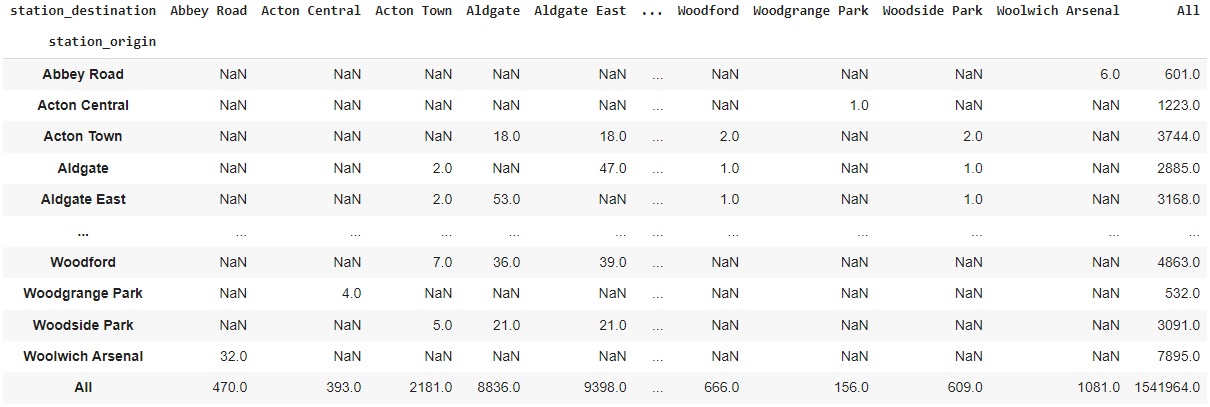
\includegraphics[width=16cm]{Image/Part2_OD4_scenario A.png}
        \caption{Scenario A}
        \label{fig:Part2_OD4_scenario A}
    \end{figure}

\newpage    

\subsubsection{Scenario B}

\textbf{Measure 1}

Assuming an increase in cost, which in this model refers to distance, two scenarios were simulated. The first scenario involved a 30\% increase, while the second involved a 50\% increase. Simulations were also conducted with a 10\% increase, but there were limitations in validating the results. Therefore, more significant increases were chosen to evaluate the system's behaviour. In the simulation assuming a 30\% increase in cost, an equilibrium was achieved in the estimated flows of origin and destination, with flow values around 600, without impacting the total number of flows.

    \begin{figure}[htp]
        \centering
        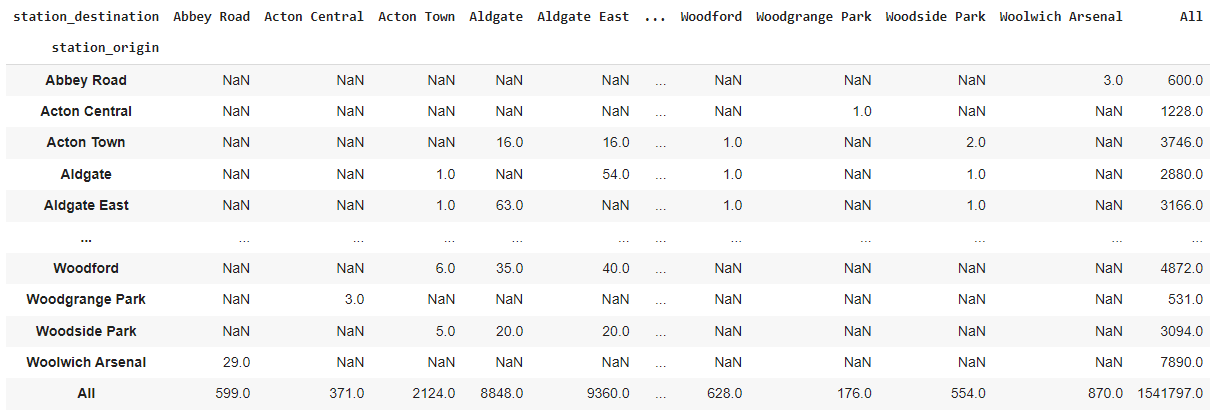
\includegraphics[width=16cm]{Image/Part2_OD6_scenario B.png}
        \caption{Measure 1 - Reducing 30\%}
        \label{fig:Part2_OD6_scenario B}
    \end{figure}

\textbf{Measure 2}    


    \begin{figure}[htp]
        \centering
        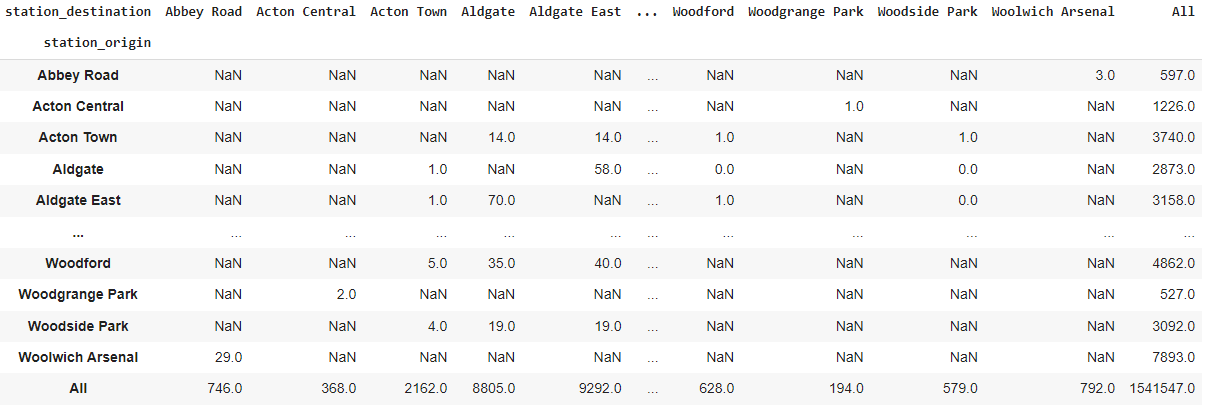
\includegraphics[width=16cm]{Image/Part2_OD8_scenario B.png}
        \caption{Measure 1 - Reducing 50\%}
        \label{fig:Part2_OD8_scenario B}
    \end{figure}

\newpage    

\subsubsection{Discussion}













% -------------------  BIBLIOGRAPHY ---------------------
\newpage
\printbibliography[title = {References}]
\addcontentsline{toc}{chapter}{References} % Adds References Section to Table of Contents


\end{document}
%  -------------------------------------------------
%  --------- The document ends from here ----------- 
%  -------------------------------------------------